\chapter{Document viewers}\label{chap:viewer}

Since now we have several text collections with different structures, we have to deal with several text viewers. By their design, all document viewers derive from a common ancestor. This means there are some features common to all viewers. Some functions work in the same way across different viewers, such as display style and word lookup. Some collections share only the same structure, but different in details. We will talk about these common features first before going into each specific viewer.

\section{Common features of document viewers}

\subsection{Three panes of the viewers}

Most viewers, in their full display, have three areas: (1) main pane at the center showing textual content, (2) navigation pane at the left used for jumping to a specific point, and (3) information pane at the right showing document information.

The first two areas are always present, but the navigator is not shown by default (except in SuttaCentral Reader). The information area may be absent in some collections that have little data. In some cases, extra information may be added into the main area, for example, the viewers of PTST and grammar books.

\dothis{To toggle the left pane, click {\ppicons A} button. To toggle the right pane, if available, click {\ppicons B} button. To toggle between full reading area and with side panes, click {\ppicons C} button.
}

Figure \ref{fig:viewer-allpanes} shows a CSTR viewer with all panes visible. On the left pane, there are three options for navigation: (1) jump by headings ({\faSix \symbol{"F1DC}}), (2) jump by paragraph numbers ({\faSix \symbol{"F1DD}}), and (3) jump by stanzas ({\faSix \symbol{"F001}}). Note that other viewers may have options similar or different to these. When clicking on the list below, you will go to the point selected.

\begin{figure}[!hbt]
\centering
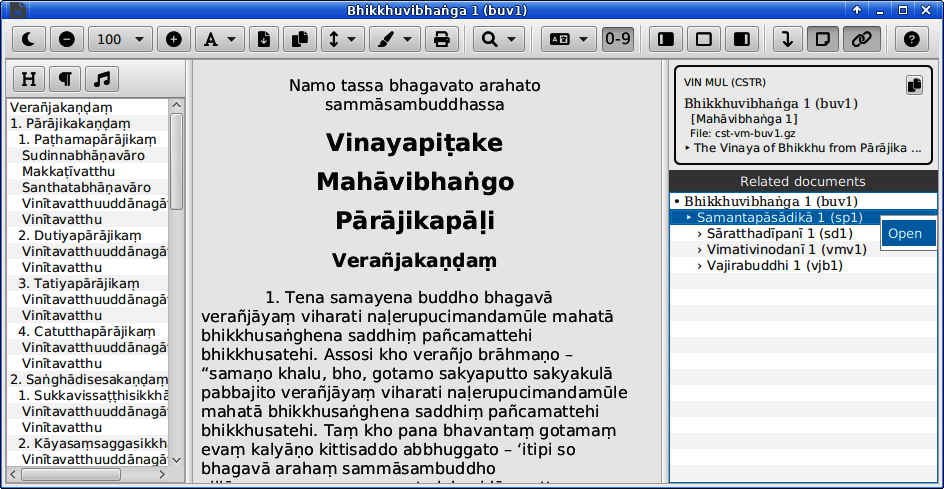
\includegraphics[width=0.9\linewidth]{images/viewer-allpanes.png}\\
\caption{CSTR viewer with all panes opened}
\label{fig:viewer-allpanes}
\end{figure}

On the right pane of this viewer (the most informative one), you can see some essential information about the document. I will not explain the detail here. You need time to be familiar with it. The most useful part of the right pane is the section of \emph{Related documents}. You can open a related text by clicking an item. Moreover, particularly with the CSTR viewer, the documents opened in this way can be synchronized together by paragraph numbers (see below).

\subsection{Word lookup}

Dictionary lookup is a very helpful tool when we read a Pāli text. All viewers or readers in the program are armed with this capability. Before you can use is feature, Dict data have to be created first (see Chapter \ref{chap:dict}). Or better, to obtain the best experience in text reading, it is highly recommended that the DPD should be installed (see Chapter \ref{chap:dpd}), otherwise the lookup will be very limited.

Once you have installed the DPD, make sure that the option of DPD integration in the Settings is selected (see Figure \ref{fig:dpd-integration}).

\begin{figure}[!hbt]
\centering
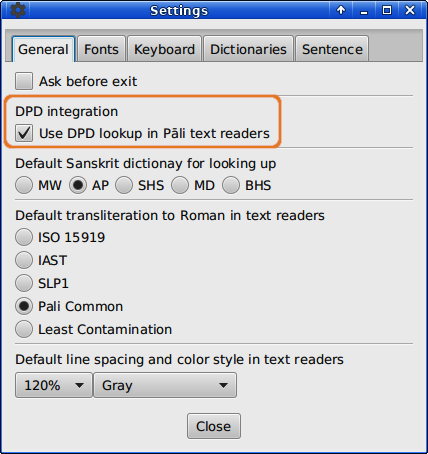
\includegraphics[width=0.6\linewidth]{images/dpd-integration.png}\\
\caption{The option of DPD integration in Settings}
\label{fig:dpd-integration}
\end{figure}

When dictionaries are ready, what you have to do is selecting a portion of text, typically a word (if you do not select the whole word, only the selected part is looked up). The result of the lookup will show on the upper right corner of the viewer (see Figure \ref{fig:viewer-lookup-dpd}). If nothing is found in DPD, the fallback result will come from CPED (see Figure \ref{fig:viewer-lookup-fallback}). In this fallback result, if the exact match is not found, the closest word will show up instead, marked by an asterisk (*).

\begin{figure}[!hbt]
\centering
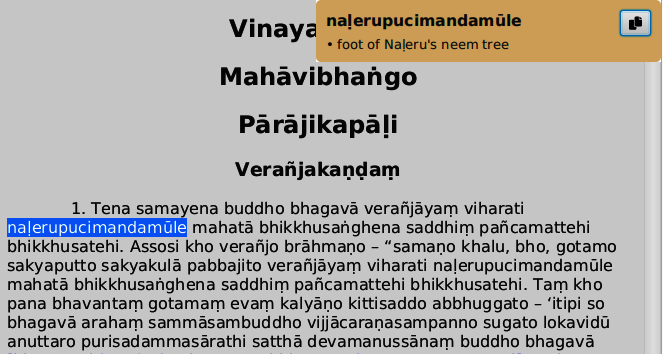
\includegraphics[width=0.9\linewidth]{images/viewer-lookup-dpd.png}\\
\caption{Word lookup with DPD integration}
\label{fig:viewer-lookup-dpd}
\end{figure}

\newpage
\boxnote{Note that in DPD searching, it finds the exact word as selected. Even though the DPD has a massive word list, and it is likely that you can find what you are looking for, it may fail with a partial word.\\
\hspace{5mm}If nothing comes up from DPD, the program searches further in CPED. With this fallback lookup, if the exact word is not found, the program tries its best guess with the closest result. If you see an asterisk (*), it means the result can be irrelevant, but some information may be helpful.}

\begin{figure}[!hbt]
\centering
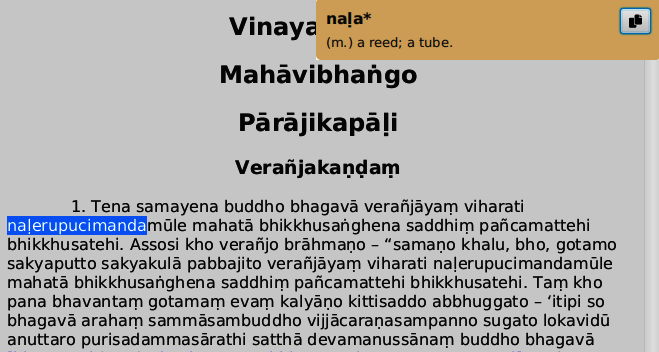
\includegraphics[width=0.9\linewidth]{images/viewer-lookup-fallback.png}\\
\caption{Word lookup with a fallback result}
\label{fig:viewer-lookup-fallback}
\end{figure}

\newpage
\subsection{Finding a string}

When reading a document, you have a good chance to find a specific string. So, a simple text searching tool is necessary in viewers. All viewers here use the same search widget. You can invoke the search tool by simply pressing \texttt{Ctrl-F} or use {\faSix \symbol{"F002}} menu button.

\dothis{Useful shortcuts for searching a string:\\
\hspace{5mm}\bullet\ \texttt{Ctrl-F} opens the search tool.\\
\hspace{5mm}\bullet\ \texttt{Ctrl-G} goes to the next occurrence.\\
\hspace{5mm}\bullet\ \texttt{Ctrl-Shift-G} goes to the previous occurrence.
}

The search function is quite effective but with some limitation. You do not need to enter characters with diacritical marks. Just type in a plain English word, then the program will find the closest ones to you. See Figure \ref{fig:viewer-stringsearch} for an example. You can force strict diacritical search, including case sensitivity, by toggle the {\faSix C} button. One limitation of the search is it cannot find a whole word (a string with word boundaries). It normally searches a string in any part. Another limitation is it cannot search with a regular expression.

\boxnote{The string search is aware of diacritics, including formatted quotation marks. So, just type a simple word and see the result.\\
\hspace{5mm}If an exact diacritical character is needed, enable \emph{case sensitive} option by toggling the {\faSix C} button.
}

\begin{figure}[!hbt]
\centering
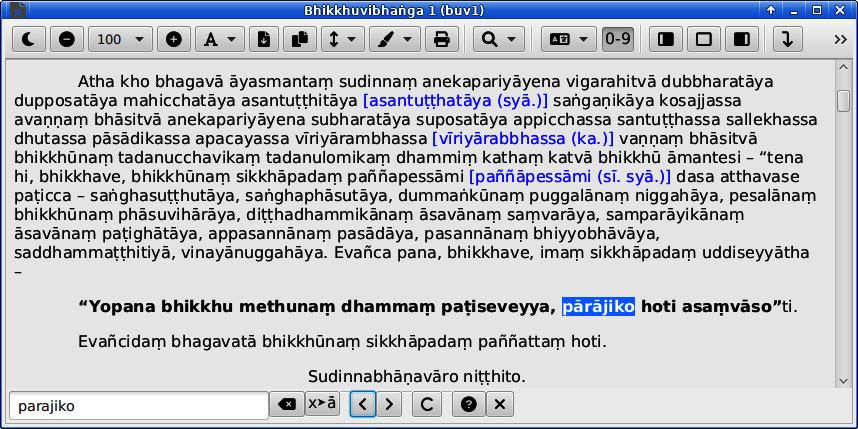
\includegraphics[width=0.9\linewidth]{images/viewer-stringsearch.png}\\
\caption{String search in viewers}
\label{fig:viewer-stringsearch}
\end{figure}

\newpage
\subsection{Context menu}

Context menu is a menu that shows up when you right-click the mouse. This can lead to some useful functions that unable to access by other ways. In all viewers, this context menu shares the same functionality. Once you select a part of text and right-click, you will see a menu as shown in Figure \ref{fig:viewer-contextmenu}.

Here are explanations on the menu:

\begin{compactitem}
\item \textbf{Open in text editor} will open the portion selected in a new instance of the program's Text Editor. The text can be processed further with various tools there (see Chapter \ref{chap:editor}).
\item \textbf{Read this portion} will open the portion selected in Sentence Reader (see Chapter \ref{chap:sentreader}).
\item \textbf{Open Pāli Dictionaries} will open the first word selected in a new instance of Pāli Dictionaries (see Chapter \ref{chap:dict}).
\item \textbf{Open Sanskrit Dictionaries} is like the previous one but Sanskrit Dictionaries will be opened.
\item \textbf{Send to Pāli Dictionaries} will send the first word selected to the Pāli Dictionaries tab in the main window.
\item \textbf{Send to Sanskrit Dictionaries} is like the previous one but the Sanskrit Dictionaries tab will be the target.
\item \textbf{Calculate meters} will calculate prosodic meters of the portion in a new instance of the program's Text Editor.
\item \textbf{Analyze this stanza/portion} will analyze the portion with the Prosody window (see Chapter \ref{chap:prosody}).
\end{compactitem}

\begin{figure}[!hbt]
\centering
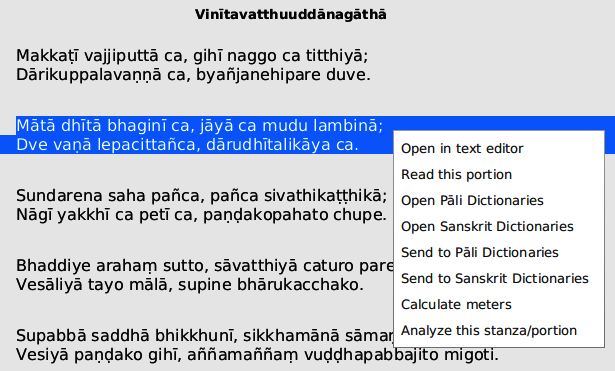
\includegraphics[width=0.9\linewidth]{images/viewer-contextmenu.png}\\
\caption{Context menu in text viewers}
\label{fig:viewer-contextmenu}
\end{figure}

\subsection{Script transformation}

Most text corpora in \textsc{Pāli\,Platform}, except the CST Devanāgarī base, are in Roman script. That is enough in most cases for Pāli studies. However, in some learning or redacting contexts you may want to see the texts in a different script. Script transformation is available to all collections, except PTST, and SKT documents.\footnote{The texts in PTST are highly contaminated with English. So, the transformation cannot be done cleanly. Also Sanskrit documents from GRETIL are of great varieties and contamination. However, texts once viewed in a reader can be selected and opened in Text Editor. The portion can always be converted there.}

If the transformation is available, you will see {\faSix \symbol{"F1AB}} menu button. By this menu, you can select one of six scripts: Roman, Devanagari, Khmer, Myanmar, Sinhala, and Thai. Figure \ref{fig:viewer-khmer} shows a document converted to Khmer script.

\begin{figure}[!hbt]
\centering
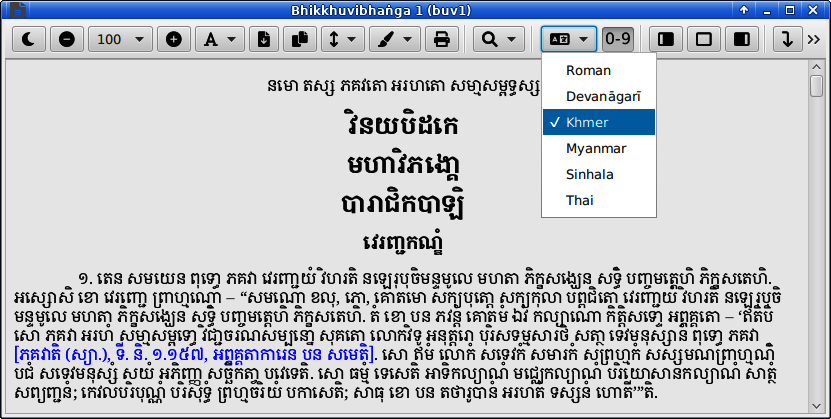
\includegraphics[width=0.9\linewidth]{images/viewer-khmer.png}\\
\caption{A document in Khmer script}
\label{fig:viewer-khmer}
\end{figure}

\boxnote{Some scripts have their own rendition of numbers. To enable number transformation, use \textbf{0-9} toggle button.}

If you work on the collection of CST Devanāgarī, it is likely that you may need to convert the text to Roman script. Or you may have some non-Roman text and you need a Roman version of it. In these use cases, you have to know about Roman transliteration.

In text viewers, when you convert text to Roman, if you use CST Devanāgarī, the default method of transliteration is preset in the Settings (see Figure \ref{fig:settings-roman}).\footnote{This setting is effective only when converting Devanāgarī text in CST Deva corpus to Roman. For other corpora, when the Roman text is seen, the viewers just restore its original, which may be of different transliteration methods.} For the differences, see Chapter \ref{chap:basic}. You have to be aware of this before making use of the Roman result.

\begin{figure}[!hbt]
\centering
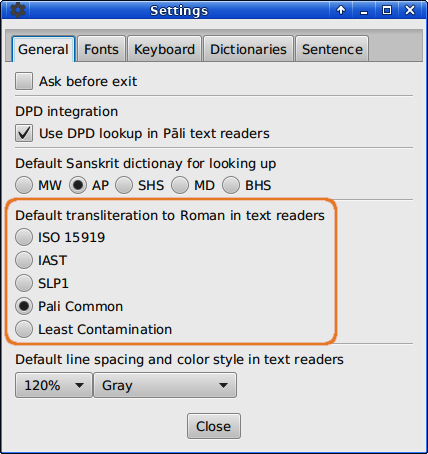
\includegraphics[width=0.6\linewidth]{images/settings-roman.png}\\
\caption{Default Roman transliteration in text viewers}
\label{fig:settings-roman}
\end{figure}

\subsection{Style and formatting}

In text viewers, we have limited options of style and formatting. Only two things can be set: (1) color style, and (2) line spacing. We have some options of text/background color under {\faSix \symbol{"F1FC}} menu button. And line spacing can be set by percentage using {\faSix \symbol{"F07D}} menu button. Figure \ref{fig:viewer-style} shows a viewer in blue background with 200\% spacing.

\begin{figure}[!hbt]
\centering
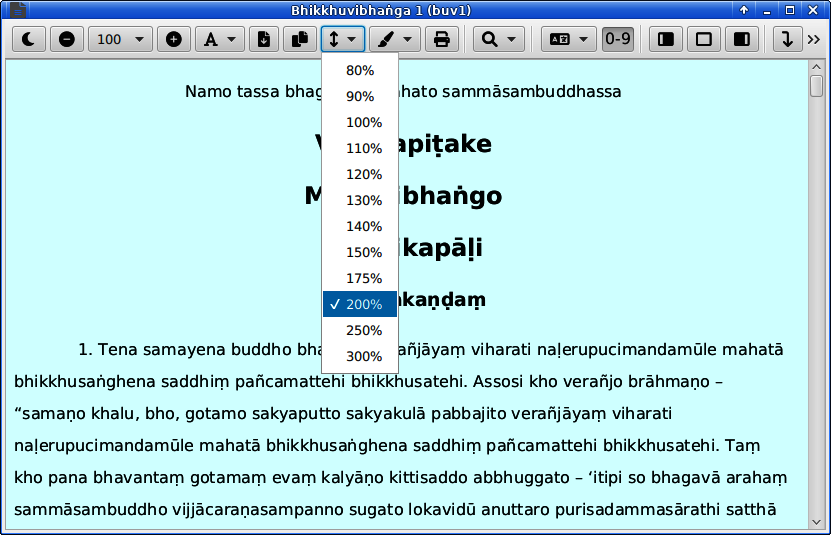
\includegraphics[width=0.9\linewidth]{images/viewer-style.png}\\
\caption{Style settings in a text viewer}
\label{fig:viewer-style}
\end{figure}

Setting the options every time you open a text is not convenient. So, we have default settings for line spacing and color style as shown in Figure \ref{fig:settings-style}.

\begin{figure}[!hbt]
\centering
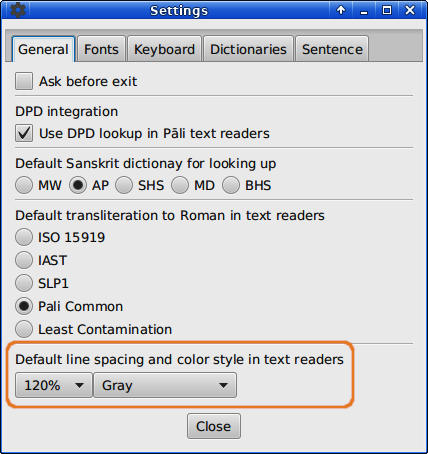
\includegraphics[width=0.6\linewidth]{images/settings-style.png}\\
\caption{Default line spacing and color style}
\label{fig:settings-style}
\end{figure}

\subsection{The last jump}

I think this function is the least known and the users often overlook it, but it can make life a little easier. So, I add this section here in short.

When you navigate the text with the left pane and the viewer goes to the point you have selected, once you close the left pane, the text does not stay in place where it should be. To solve this problem, you just click the {\faSix \symbol{"F149}} button and the viewer will go to the place you have selected before.

\section{Specific features in various viewers}

In the following part I will explain some specific features available only in some viewers.

\subsection{Synchronization in CST Restructured}

This is a unique feature of this corpus. I spent several months to make this possible. In a nutshell, synchronization means when you open a text with related documents (using the right pane described above), once you go to a specific paragraph (using paragraph number navigator on the left pane) on the main text, all related documents opened will move to the same paragraph number. This is very useful when you seriously read a Pāli text with its commentaries. Figure \ref{fig:viewer-synch} has a demonstration of this feature.

\begin{figure}[!hbt]
\centering
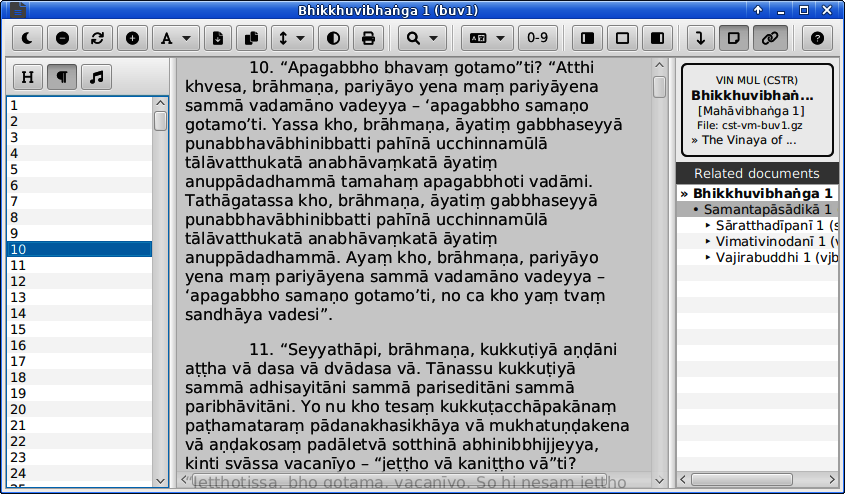
\includegraphics[width=0.9\linewidth]{images/viewer-synch-main.png}\\
(a) A paragraph number is selected in the main text\\[3mm]
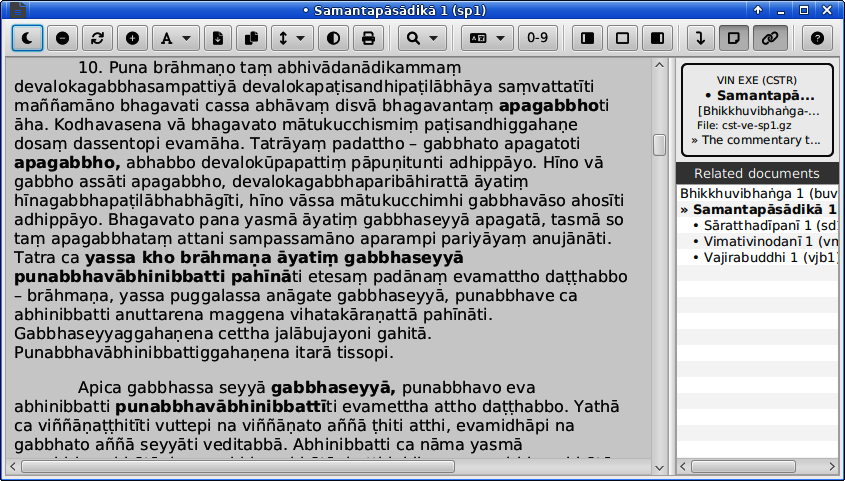
\includegraphics[width=0.9\linewidth]{images/viewer-synch-related.png}\\
(b) The related text opened jumps to the same number\\
\caption{Synchronization between CSTR viewers}
\label{fig:viewer-synch}
\end{figure}

\newpage
\boxnote{The synchronization can be done when {\faSix \symbol{"F0C1}} toggle button is pressed, and the related documents have to be opened with the right pane (not by TOC Tree).\\
\hspace{5mm}Even though you can open a related document likewise in CST4 and BJT collection, the texts opened cannot be synchronized because this part of data is not available in other collections.}

\subsection{Notes and publication references}

If a collection has notes in its texts (either footnotes or inline notes that have a kind of detectable structure), this part of notes can be turned on and off by {\faSix \symbol{"F249}} toggle button. These notes are usually formatted with a different color, often placed within brackets.

In CST Deva and CST4 collection, information about publication references is also available.\footnote{CST Devanāgarī and CST4 data customized have identical structure, so they use the same viewer.} This part of information is unique to these corpora. Even if it has little use nowadays, it is kept for a historical reason. To see publication references, enable {\faSix \symbol{"F292}} toggle button. Figure \ref{fig:viewer-notesref} shows a text in CST4 collection with notes and references visible.

\begin{figure}[!hbt]
\centering
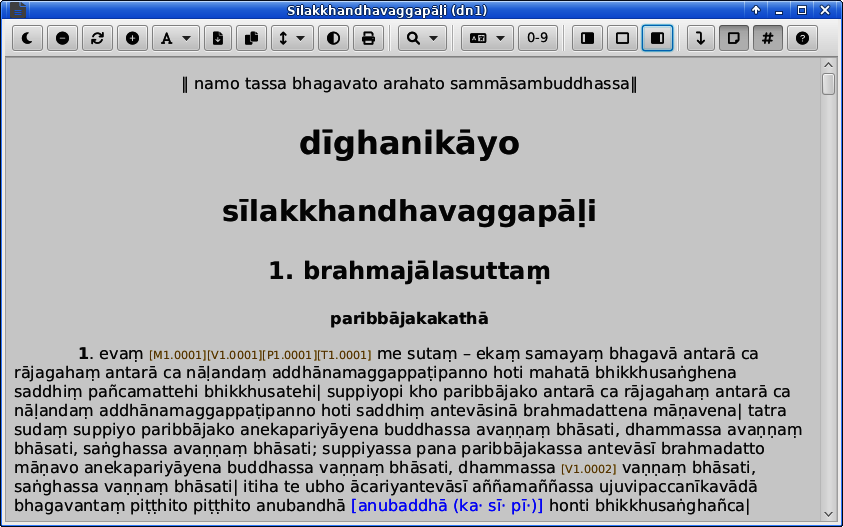
\includegraphics[width=0.9\linewidth]{images/viewer-notesref.png}\\
\caption{A document with notes and publication references}
\label{fig:viewer-notesref}
\end{figure}

\subsection{Information and format in PTST viewer}

Because texts in the collection of PTS come from GRETIL, they have some information attached. This information looks intrusive in the original. So, it is hidden in the viewer. To see the information, you can use two buttons at the top of the viewer (see Figure \ref{fig:viewer-pts}). The buttons are pale to make them less distracting, but they are clickable. 

\begin{figure}[!hbt]
\centering
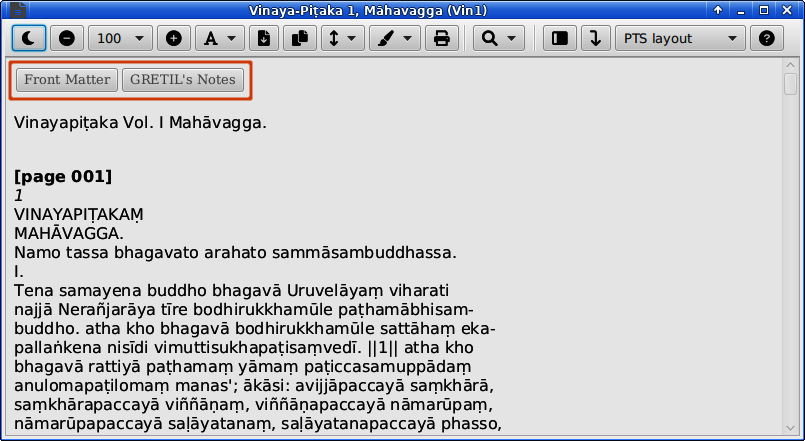
\includegraphics[width=0.9\linewidth]{images/viewer-pts.png}\\
\caption{Buttons for text information in PTST viewer}
\label{fig:viewer-pts}
\end{figure}

Another unique characteristic of texts in PTST collection is they have two layouts available: (1) PTS layout, and (2) floating text. The former is like pages in the book version. So, you can see a lot of hyphenations. The latter is an attempt to eliminate those hyphenations by making terms connected. This can also ease string searching.

When you want to see the original layout, use the first option. If you want to find a string in the text, use the second. Figure \ref{fig:viewer-pts-float} show a document of PTST in floating text.

\begin{figure}[!hbt]
\centering
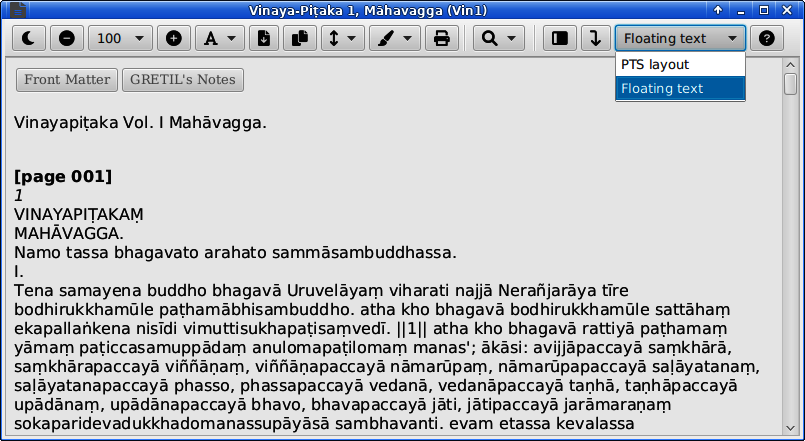
\includegraphics[width=0.9\linewidth]{images/viewer-pts-float.png}\\
\caption{Floating text layout in PTST viewer}
\label{fig:viewer-pts-float}
\end{figure}

\subsection{Dehyphenation in SRT viewer}

Texts in SRT collection are also in book layout. This makes some long words broken by hyphenation. You can connect those words by using {\faSix \symbol{"F7D9}} button. The dehyphenation is done by calculation. It is good enough but not perfect. You may come across an odd result from a borderline case. Figure \ref{fig:viewer-srt} show a result of dehyphenation in this viewer.

\begin{figure}[!hbt]
\centering
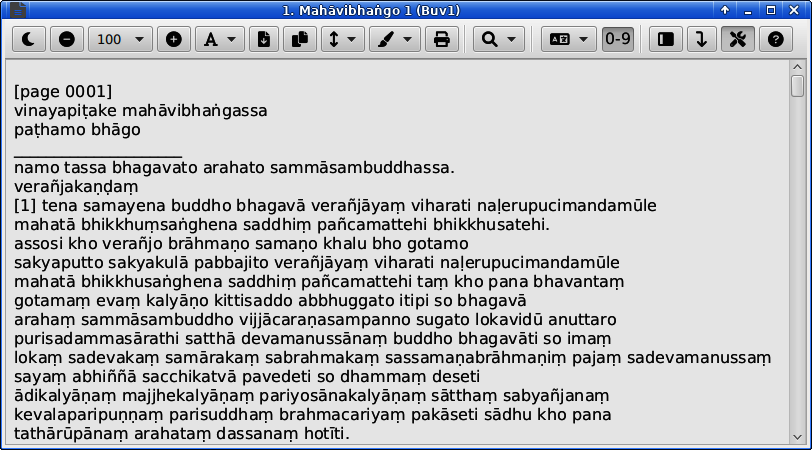
\includegraphics[width=0.9\linewidth]{images/viewer-srt.png}\\
\caption{Dehyphenation in SRT viewer}
\label{fig:viewer-srt}
\end{figure}

\subsection{Viewer of Kaccāyana}

This is the best representation of the viewer for Pāli grammar books. In this collection, a book with its related works can be viewed together. Books that can be put in parallel must have the same running numbers that can be linked together. And Kaccāyanabyākaraṇa have several commentaries available making this feature really helpful.\footnote{The viewer of Moggallānabyākaraṇa can do likewise. Abhidhānappadīpikā and its ṭīkā can also do the same.}

Figure \ref{fig:viewer-kacc} shows Kaccāyana with Rūpasiddhi as a related work. You can add other books likewise by the options provided. Note that only related suttas are brought here. For the text outside the suttas, you have to open the books directly to see it.

\begin{figure}[!hbt]
\centering
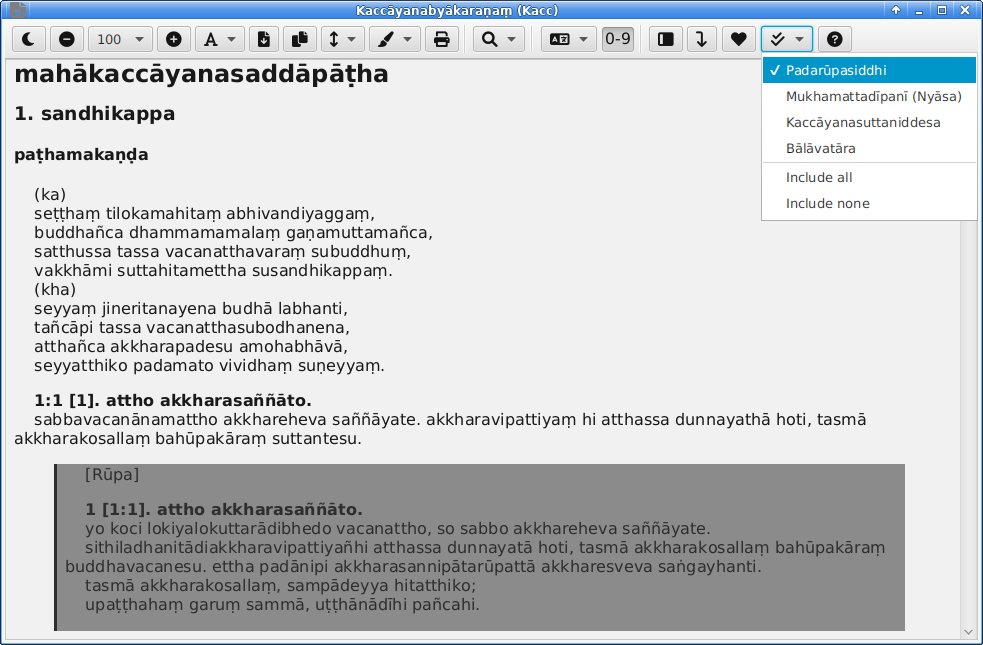
\includegraphics[width=0.9\linewidth]{images/viewer-kacc.png}\\
\caption{Viewer of Kaccāyana viewed together with Rūpasiddhi}
\label{fig:viewer-kacc}
\end{figure}

In this viewer, you can see only the head of suttas by toggle {\faSix \symbol{"F08A}} button. Figure \ref{fig:viewer-kacc-head} show the head of suttas with all related books added.

\begin{figure}[!hbt]
\centering
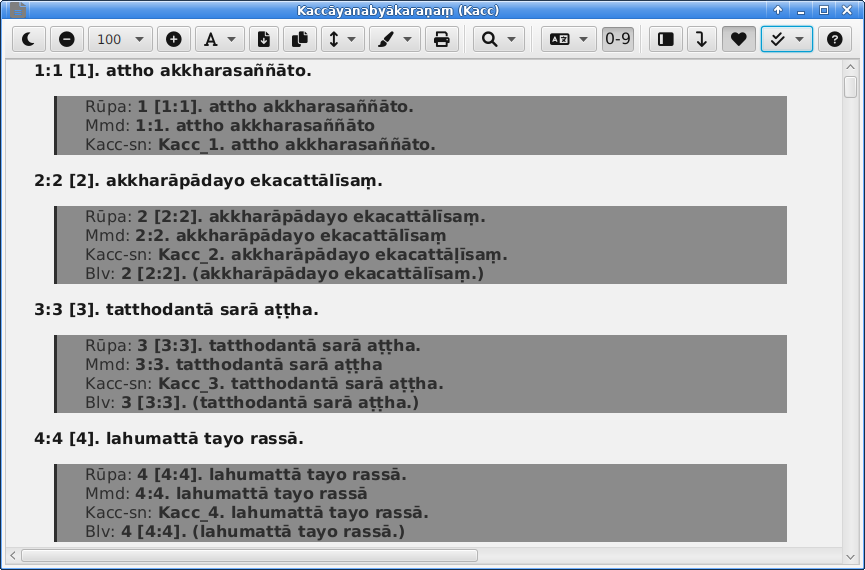
\includegraphics[width=0.9\linewidth]{images/viewer-kacc-head.png}\\
\caption{Suttas of Kaccāyana with all related works}
\label{fig:viewer-kacc-head}
\end{figure}

\subsection{SuttaCentral Reader}

If you install the text collection from SuttaCentral, the viewer for this corpus will be available. You can open this viewer by clicking {\ppicons S} button or using menu Reader > {\ppicons S} SuttaCentral Text Reader.

\newpage
\dothis{You can download the recent text collection of SuttaCentral by menu Reader > {\faSix \symbol{"F381}} Download SuttaCental data. The downloader has similar functions as the DPD downloader (see Chapter \ref{chap:dpd}).\\
\hspace{5mm}Once the collection zip file is available, press {\ppicons S} button to open the reader.
}

The viewer of SuttaCentral is quite powerful. It can show most information of texts available in the corpus, including translations and other information.\footnote{Still, many information unrelated to the texts are left out. Please go to its site (\url{suttacentral.net}) directly for such information.} I will not explain this viewer more than this. It is on the user's part to find out by experimenting (the best way to learn). Figure \ref{fig:viewer-suttacentral} shows a document in SuttaCentral collection with full options.

\newpage
\begin{figure}[!hbt]
\centering
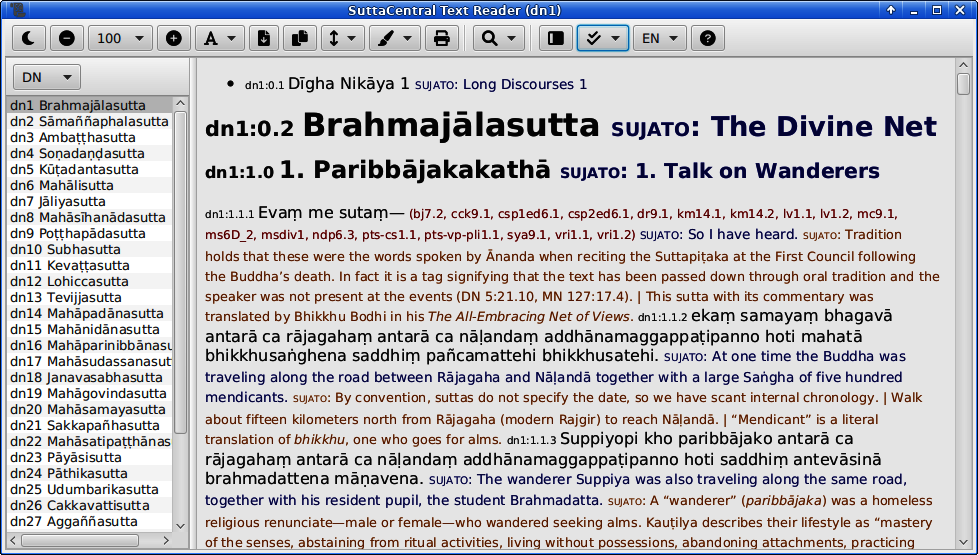
\includegraphics[width=0.9\linewidth]{images/viewer-suttacentral.png}\\
\caption{SuttaCentral viewer in full options}
\label{fig:viewer-suttacentral}
\end{figure}

